% Encodage du fichier : UTF-8
% Conserver empty -> pas de numéros de pages
\documentclass[empty]{fjc2014} %[cropmarks] 
\usepackage{microtype}
\usepackage{graphicx}
\usepackage{hyperref}

\submitted{FJC 2025}{1}

\title[fjc]{Développement d'un framework de suivi et d'évaluation de l'impact à travers un data warehouse sémantique pour les méta-organisations}

\author{Clément Combier}

\address{%
Université de Pau et des Pays de l'Adour \\
E2S-UPPA, LIUPPA\\
1 Allée du Parc Montaury\\
64600, Anglet, France\\[6pt]
clement.combier@univ-pau.fr} 


\motscles{data warehouse, web sémantique, méta-organisation, étude d'impact, mesure d'impact, système de suivi et d'évaluation, étude du management, théorie du changement}
\keywords{data warehouse, semantic web, meta-organisation, impact study, impact evaluation, monitoring and evaluation system, management study, theory of change}
\resume{Adèl Nourredine, Jose Enrique Armendariz-Inigo, Phillipe Arnould}

\begin{document}\maketitlepage
\section{Contexte}
Les méta-organisations, définies comme des groupements d'organisations autour d’objectifs communs, émergent dans des domaines variés : académique, industriel, territorial, etc. Leur gouvernance distribuée, la diversité de leurs membres, et la multiplicité de leurs projets rendent l’évaluation de leur impact complexe. Cette étude propose un framework générique de suivi et d’évaluation de l’impact (S\&E) adapté à ces structures. Notre proposition intègre des technologies sémantiques au sein d’un data warehouse pour faciliter l’agrégation, l’interprétation et l’exploitation de données hétérogènes issues de plusieurs organisations.
Ce travail est expérimenté dans le cadre de l’alliance universitaire européenne UNITA, utilisée ici comme cas d’usage représentatif d’une méta-organisation, sans en restreindre la portée générale.

\section{État de l'art}
La concentration sur les alliances universitaires a fortement augmenté depuis le lancement en 2019 de l'Initiative des Universités Européennes (IUE). À mesure que ces partenariats se développent, il est crucial d'évaluer leur impact sociétal et de formuler des stratégies de suivi complètes. Cette analyse explore la recherche axée sur la mesure de l'impact, la Théorie du Changement (TdC) et les systèmes de Suivi et d'Évaluation (S\&E) au sein de méta-organisations comme les alliances universitaires. En investiguant ces sujets, nous visons à établir un cadre solide pour évaluer leur impact.  Nous avons séparé l'étude en deux axes majeurs que nous allons explorer dans deux parties de cet état de l'art. La première section se concentre sur l'étude d'impact et la théorie du changement, fortement liées. Puis, les systèmes de suivi et d'évaluation automatisés orientés données pour la partie plus technique de la recherche.

%Add a subsection on meta-organisations
\subsection{Étude d'Impact et Théorie du Changement}
%\begin{figure}
%    \centering
%    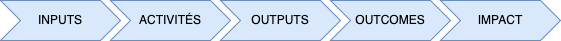
\includegraphics[width=0.75\linewidth]{images/Diagrams-IMPACT.png}
%    \caption{Chaîne d'impact simplifiée \cite{peersman_when_2016}}
%    \label{fig:simplified-impact-chain}
%\end{figure}
Le terme ‘impact’ fait souvent référence aux effets à long terme des activités sur leur environnement. Nous adoptons la définition du Comité d'Aide au Développement (CAD) de l’Organisation de Coopération et de Développement Économiques (OCDE) : "les effets à long terme positifs et négatifs, primaires et secondaires, produits par une intervention de développement, directement ou indirectement, intentionnels ou non." \cite{oecd_quality_2010}.  
L'impact étudié dans ce travail est conçu comme global et multidimensionnel, regroupant des effets organisationnels, sociétaux, académiques, économiques et culturels, selon les objectifs propres à chaque méta-organisation. Ce choix de structure permet au framework de rester flexible et adaptable à différents types de projets ou contextes. Les indicateurs sont choisis en fonction des priorités de l’organisation analysée, tout en respectant un canevas unifié. Un outil souvent utilisé dans l'étude d'impact est la chaîne d'impact simplifiée comme expliqué par \cite{peersman_when_2016}. Elle se compose des inputs, en entrées qui seront utilisés pour différentes activités et actions. Puis, en résultat de ces actions, nous aurons des outputs, qui mènent à un plus haut niveau aux outcomes de l'action, puis en fin de chaîne nous avons l'impact de nos actions. 
%La figure \ref{fig:simplified-impact-chain} présente une chaîne d'impact simplifiée reliant les ressources, activités, résultats et effets \cite{peersman_when_2016}.

La théorie du changement a évolué au fil du temps, débutant avec le "Modèle de Changement en Trois Étapes" de Kurt Lewin \cite{lewin_frontiers_1947} et se développant à travers des modèles cycliques élargis par Lippitt et al. \cite{lippitt_dynamics_1958} et Prochaska et DiClemente \cite{prochaska_stages_1983}. Ces théories, semblables à la Théorie de l’Action Raisonnée et du Comportement Planifié, intègrent des notions clés comme "le contrôle perçu", mais manquent d'une perspective sociétale. Nous examinons la théorie du changement dans le domaine de l'Alphabétisation Politique, fusionnant une approche politiquement informée et stratégique, cruciale pour planifier, suivre et évaluer les changements au sein des méta-organisations. Elle nous permet, entre autres, d'utiliser le concept de la Narration du Changement pour planifier l'étude d'impact.

\subsection{Système de Suivi et d'Évaluation automatisé orienté données}
Les systèmes de Suivi et d'Évaluation (S\&E) combinent des évaluations régulières pour des mesures quantitatives avec une surveillance continue pour identifier les anomalies, assurant des données fiables tout au long du cycle de vie d’un projet. Avec notre approche orientée données, nous nous intéressons au cadre proposé et faisons le lien avec la sous-section suivante.
Les entrepôts de données orientés vers la connaissance centralisent et exploitent des informations souvent abstraites comme l’impact sociétal. Ils fournissent une perspective unifiée au sein de la méta-organisation, facilitant des évaluations précises grâce à des indicateurs statistiques.
Dans notre cas, nous proposons un entrepôt de données sémantique intégrant les technologies du Web sémantique (ontologies, RDF, SPARQL) pour améliorer l’interopérabilité entre sources hétérogènes, la compréhension machine des données et leur contextualisation. 

\section{Problématique}
De nombreux frameworks et méthodologies ont été développés et proposés au fil des ans sur la théorie des changements et  d'évaluation de l'impact. Cependant, ces cadres peuvent ne pas fournir aux méta-organisations les outils et la flexibilité des organisations simples. Ceci prouve l'importance d'une méthodologie plus large pour les méta-organisations, tout en gardant une ancre pour chaque organisation partenaire.
Ce projet de recherche vise à développer un cadre pour les méta-organisations (dans ce contexte, les alliances d'universités européennes) pour surveiller et évaluer leur impact sur la société en utilisant des solutions orientées données. 

\section{Actions réalisées}
Notre initiative s'aligne avec le collectif universitaire européen, UNITA - Universitas Montium, qui regroupe 12 établissements académiques dédiés à la poursuite d'objectifs communs. Cette alliance sert de terrain d'essai audacieux, mettant en avant les obstacles que doivent surmonter les universités européennes — et plus largement, les méta-organisations — pour évaluer leur impact sociétal. Notre stratégie repose sur un cadre pluridimensionnel qui aide les méta-organisations comme UNITA à mesurer leur influence grâce à des méthodologies basées sur les données et des outils analytiques. Nous avons développé une solution de stockage orientée impact qui intègre la collecte de preuves, l'analyse d'indicateurs, et des entretiens collectifs. Au cœur de cette méthode se trouvent les indicateurs de production (résultats immédiats, comme le nombre de projets réalisés) et les indicateurs de résultats (effets à moyen terme, tels que de meilleures opportunités de collaboration) qui jouent un rôle clé dans le suivi des progrès et le soutien des décisions stratégiques. Notre méthode se déploie en trois étapes distinctes : \textbf{ (1) Discussion} : Déterminer les besoins spécifiques de chaque membre. \textbf{(2) Évaluation} : Valider l'adéquation et la fiabilité des indicateurs clés. \textbf{(3) Construction} : Intégrer les données validées dans un Entrepôt de Données (DW). 

Au cours de cette première année, nous avons adopté une méthodologie bien organisée pour rassembler les indicateurs et les besoins spécifiques aux différents travaux de l'alliance UNITA. Par le biais d'entretiens collaboratifs, nous avons dressé et approuvé une liste d'indicateurs clés en étroite collaboration avec chaque équipe. Cette étape aboutit à travers une seconde série d'entretiens spécialement dédiée à la validation des données. Une fois les données purgées de toute incohérence et doublon, elles se trouvent intégrées dans un DW centralisé. Ce dispositif simplifie le suivi des avancées, la détection des grandes lignes et la prise de décisions stratégiques éclairées. Après validation, chaque indicateur est prêt à être collecté auprès des institutions membres pour initier les analyses telles que l'élaboration de rapports et la prévision de l'impact. 



\section{Actions futures}
Nous sommes en train d'implémenter les indicateurs recueillis lors des interviews. Avec les données obtenues, nous avons  une vision des sources de données d'où nous pouvons extraire les informations nécessaires au calcul des indicateurs sélectionnés par les différentes tâches du projet. 
L'implémentation se fait en plusieurs étapes. La première consiste à fournir une entrée utilisateur directe pour la saisie d'indicateurs bruts calculés manuellement. Cette initiale implémentation permet de commencer le suivi le plus tôt possible pendant la mise en place du processus et du pipeline de données. 
Une fois cette première implémentation effectuée, nous allons travailler par tiers sur un an pour intégrer progressivement et tester le système et les méthodes de calcul pour nos indicateurs d'outputs et outcomes. 
Parallèlement, l'utilisation de la Narration du Changement nous permettra de débuter l'étude d'impact le temps qu'un ensemble significatif de données ait pu être collecté. Cette narration permet d'interpréter les perspectives de chaque tâche sur leur environnement au niveau du projet, de l'alliance et de l'environnement de chaque institution de l'alliance.

% Deux possibilités pour la bibliographie : à la main ou avec BibTeX (hautement recommandé)
% pour bibtex -> remplir un fichier fjc2014.bib
% utiliser les commande \cite{bibkey2,bibkey2} et \citeasnoun{bibkey}
\bibliography{fjc2014}
\end{document}
